% Chapter Template
\chapter{CNN: implementazione e addestramento} % Main chapter title
\label{Capitolo4}
\def \path	{Figures/C4}
In questo capitolo verranno messi in pratica i concetti introdotti nel Capitolo \ref{Capitolo3}. In particolare, verrà addestrata una CNN su 2 dataset, MNIST e CIFAR. I risultati su quest'ultimo serviranno da confronto con ResNet, la rete utilizzata nel Capitolo 5. 
%--------------------------------------------------------------------
%	SECTION 1
%--------------------------------------------------------------------
\section{Modello di CNN basato su LeNet}
La rete implementata è basata sulla capostipite delle CNN, \texttt{LeNet5}, resa celebre da Y. LeCun per il riconoscimento di caratteri, anche scritti a mano\parencite{lenet}.  L'architettura è rappresentata in figura \ref{fig:lenet}. Si noti che la rete è appositamente progettata per avere in input immagini di 32x32 pixel, adatta ai dataset che si introduranno dopo. 
\begin{figure}[h!]
 \centering
 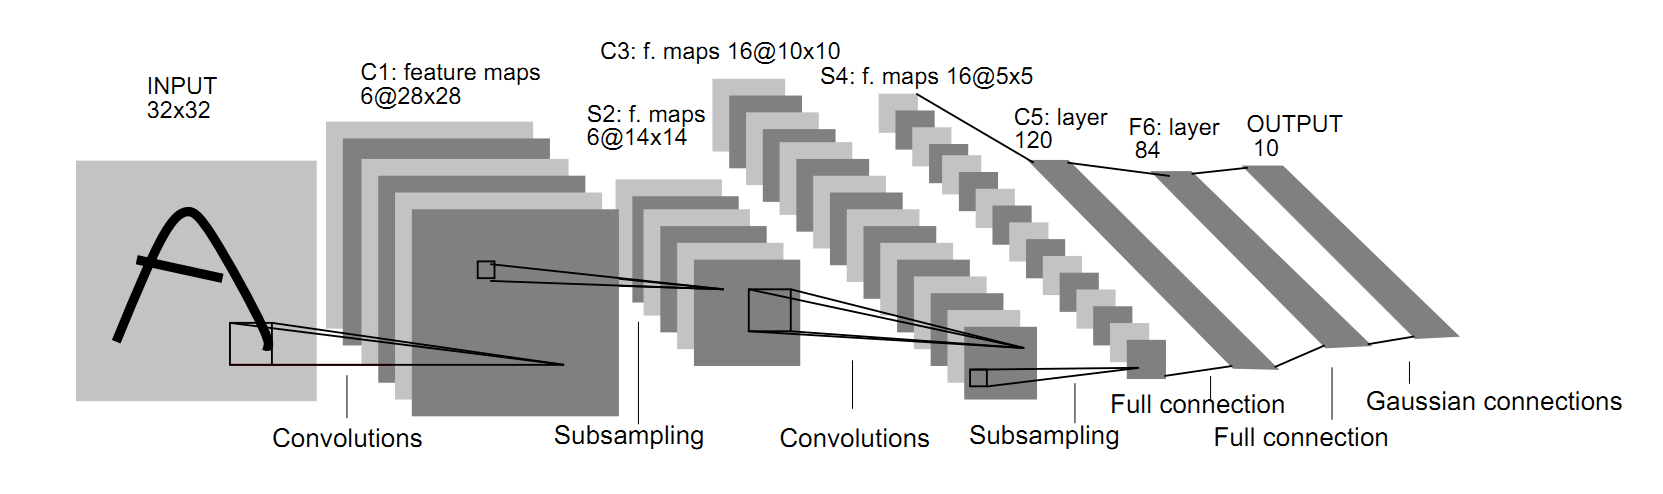
\includegraphics[width=1.0\textwidth]{\path/lenet.png} 
 \caption{Architettura di LeNet5, qui per il riconoscimento di caratteri scritti a mano}
 \label{fig:lenet}
\end{figure}	\\
Per implementare la rete verrà impiegato il già citato framework Torch. Per saperne di più su Torch e sugli utilizzi basilari per le reti neurali si veda l'appendice \ref{AppendixB}.

Si procede quindi, ad implementare la rete costituita da: 
\begin{itemize}
\item 2x $\rightarrow$ Convolutional layers - ReLU - Pooling layers
\item 1x $\rightarrow$ Multi-layer perceptron completamente connesso, con 1 hidden layer 
\end{itemize}

%% inserire codice rete %% 

\begin{lstlisting}[language={[5.2]Lua}]
--hyper-parameters
nfeats = 3               --3D input volume
nstates = {16, 256, 128} --output at each level
filtsize = 5             --filter size or kernel
poolsize = 2

--gaussian kernel for std normalization 
normkernel = image.gaussian1D(13)

-- define model to train
-- on the 10-class classification problem
---
classes = {'airplane', 'car', 'bird', 'cat',
   'deer', 'dog', 'frog', 'horse', 'ship', 'truck'}


--first, we get a sequential model onto which we'll add every layer
model = nn.Sequential()
------------------------------------------------------------
-- convolutional network
------------------------------------------------------------
-- stage 1 :  filter bank -> squashing -> max pooling -> mean+std normalization
--            3 -> 16
model:add(nn.SpatialConvolutionMM(nfeats, nstates[1], filtsize, filtsize))
model:add(nn.ReLU())
model:add(nn.SpatialMaxPooling(poolsize, poolsize, poolsize, poolsize))
model:add(nn.SpatialSubtractiveNormalization(nstates[1], normkernel))

-- stage 2 : filter bank -> squashing -> max pooling -> mean+std normalization
--           16 -> 256
model:add(nn.SpatialConvolutionMM(nstates[1], nstates[2], filtsize, filtsize))
model:add(nn.ReLU())
model:add(nn.SpatialMaxPooling(poolsize, poolsize, poolsize, poolsize))
model:add(nn.SpatialSubtractiveNormalization(256, normkernel))

-- stage 3 : standard 2-layer neural network
--           256 -> 128 -> 10 -> classification
model:add(nn.Reshape(nstates[2]*filtsize*filtsize))
model:add(nn.Linear(nstates[2]*filtsize*filtsize, nstates[3]))
model:add(nn.ReLU())
model:add(nn.Linear(nstates[3],#classes))
\end{lstlisting}

\subsection{Definire la loss function}
Ora che si ha un modello, va definita una funzione di costo da minimizzare che, come visto nel capitolo 2, sta alla base dell’apprendimento. Nel capitolo 2 però, si era definito tutto "a mano", mentre ora si usano le librerie di Torch. \\Con Torch si possono definire diverse funzioni di costo, a seconda del principio di apprendimento che vogliamo utilizzare. Come ad esempio lo scarto quadratico che però non è in generale una scelta ottimale. Una delle più convienienti per i problemi di classificazione è la \emph{negative-likelihood-log} (likelihood = funzione di verosimiglianza). La NLL necessita in ingresso di un vettori di probabilità logaritmiche normalizzate. Quindi, prima si trasforma l’output del classificatore in probabilità logaritmica aggiungendo un modulo chiamato \texttt{LogSoftMax} e poi si calcola l'errore sulla NLL. In Torch questo è molto semplice: 

\begin{lstlisting}[language={[5.2]Lua}]
--add a Log-SoftMax classifier at the end of the Net
model:add(nn.LogSoftMax())

--criterion (i.e. the loss) will be the negative-likelihood
criterion = nn.ClassNLLCriterion()
\end{lstlisting}


%--------------------------------------------------------------------
%	SECTION 2
%--------------------------------------------------------------------
\section{Procedura di training}
Prima di implementare la procedura di training occorre definire con precisione la relativa terminologia: 
\begin{itemize}
\item \emph{Batch}: insieme di esempi che si da in input alla rete e su cui si va a calcolare la media dell'errore tramite backpropagation. Se gli esempi non sono molto numeri si chiama anche "mini-batch". Solitamente è a multipli di 8 (32,64,128,256). Si veda anche il Capitolo 2, sezione \ref{sec:backprop}.
\item \emph{Pass}: un forward pass + un backward pass. In altre parole si dà qualcosa in input alla rete e si calcola l'errore tramite la backpropagation. Questo "qualcosa", può essere un solo esempio, o un mini-batch.
\item \emph{iterazioni}: un pass completo di tutti gli esempi di un batch. Nel caso di batchSize = 1, iterazione e pass assumono lo stesso significato. 
\item \emph{Epoch}: con il termine epoch si intende un pass completo di tutti gli esempi del dataset.
\end{itemize}
\\
Passiamo quindi alla definizione della procedura di training: il seguente snippet di codice mostra come implementare il training di una epoch, dopodiché basterà eseguirlo in loop per tutto il dataset. 

\begin{lstlisting}[language={[5.2]Lua}]
   -- do one epoch
   print('<trainer> on training set:')
   print("<trainer> online epoch # " .. epoch .. ' [batchSize = ' .. opt.batchSize .. ']')
   for t = 1,dataset:size(),opt.batchSize do
      -- disp progress
      xlua.progress(t, dataset:size())

      -- create mini batch
      local inputs = {}
      local targets = {}
      for i = t,math.min(t+opt.batchSize-1,dataset:size()) do
         -- load new sample
         local input = dataset.data[i]
         local target = dataset.labels[i]
         table.insert(inputs, input)
         table.insert(targets, target)
      end

      -- create closure to evaluate f(X) and df/dX
      -- i.e. forward and backward pass
      local feval = function(x)
         -- get new parameters
         if x ~= parameters then
            parameters:copy(x)
         end

         -- reset gradients
         gradParameters:zero()

         -- f is the average of all criterions
         local f = 0

         -- evaluate function for complete mini batch
         -- #inputs == size of the mini-batch
         for i = 1,#inputs do
            -- estimate f
            local output = model:forward(inputs[i])
            local err = criterion:forward(output, targets[i])
            f = f + err

            -- estimate df/dW to minimize loss function
            local df_do = criterion:backward(output, targets[i])
            --backpropagation
            model:backward(inputs[i], df_do)

            -- update confusion
            confusion:add(output, targets[i])
            
         end

         -- normalize gradients and f(X)
         gradParameters:div(#inputs)
         f = f/#inputs

         -- return f and df/dX
         return f,gradParameters
      end

	  --configure optimizer parameters
      config = config or {learningRate = opt.learningRate,
           				  weightDecay = opt.weightDecay,
            		      momentum = opt.momentum,
            			  learningRateDecay = 5e-7}
      -- optimize on current mini-batch
	  --N.B. optimMethod = 'SGD' or others
      optimMethod(feval, parameters, config)
end
\end{lstlisting}
%--------------------------------------------------------------------
%	SECTION 3
%--------------------------------------------------------------------
\section{MNIST: preprocessing}
MNIST è un dataset di cifre scritte a mano, disponibile sul sito di Y. LeCun\parencite{Wlecun}, costituito da un training set di 60000 esempi e un test set di 10000. 
\\
Le immagini sono B/N, tagliate in modo tale da avere la cifra esattamente al centro dell’immagine e una risoluzione di 32x32; per questo richiedono un pre-processing minimo. Basta utilizzare uno script per scaricare le immagini e caricarle nei tensori per il training ed il testing. Dopodiché si esegue uno step di \emph{data normalization} per standardizzare i dati, sottraendo la media e dividendo per la deviazione standard. 
$$
Z = \frac{X-\mu}{\sigma}
$$
Così si avrà un dataset con media nulla e varianza pari a 1. 

%%inserire codice per dataset MNIST %% 
%--------------------------------------------------------------------
%	SECTION 4
%--------------------------------------------------------------------
\section{MNIST: addestramento}
Quindi, utilizzando il codice della sezione precedente e lanciando un addestramento su MNIST si avranno i risultati mostrati nella \emph{confusion matrix} in figura \ref{fig:mnist-training}. 
%% altri metodi però fanno fatica %% 
\begin{figure}[h!]
 \centering
 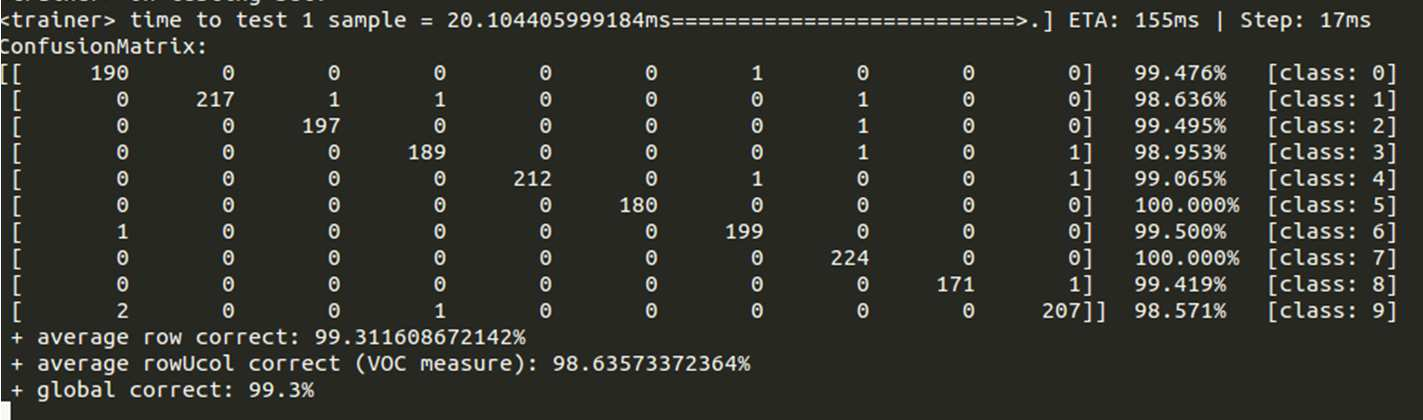
\includegraphics[width=1.0\textwidth]{\path/mnist-training.png} 
 \caption{Confusion Matrix MNIST: la matrice che mostra le percentuali di accuratezza ed errore sul test set per ogni classe}
 \label{fig:mnist-training}
\end{figure}
\\
Come da aspettative, l'architettura divenuta popolare sulla classificazione di caratteri raggiunge un'accuratezza vicina al 99.3\% in poco meno di mezz'ora di training. \\
Utilizzando una libreria per Lua basata su Javascript, si è scritto uno script per visualizzare alcune delle immagini in input durante il testing, con le rispettive classificazioni compiute dalla rete, in alto a sinistra (figura \ref{fig:mnist-correct}).
\begin{figure}[h!]
 \centering
 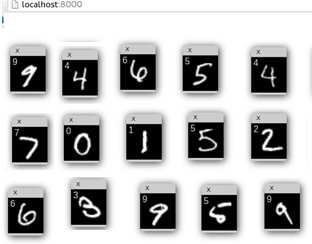
\includegraphics[width=1.0\textwidth]{\path/mnist-screen.png} 
 \caption{Esempi di cifre classificate correttamente}
 \label{fig:mnist-correct}
\end{figure}

Come dimostrato, MNIST è un dataset piuttosto semplice per le CNN. Tuttavia, è rimarchevole come in poche linee di codice si possa addestrare una rete nella comprensione dei caratteri in pochissimo tempo, laddove i metodi precedenti richiedevano più sforzi e dovevano necessariamente essere adattati e rifiniti per ogni dataset diverso. All'opposto, questa stessa CNN è stata utilizzata con successo per l'addestramento sul dataset CIFAR. 

%--------------------------------------------------------------------
%	SECTION 5
%--------------------------------------------------------------------
\section{CIFAR: preprocessing}
Il dataset CIFAR10 è decisamente più impegnativo in quanto contiene immagini a colori di 10 classi di oggetti e animali del mondo reale: aeroplani, automobili, uccelli, cani, cavalli, renne, rane, navi e camion. Vi sono 60000 immagini a colori 32x32 divisi nelle suddette 10 classi, 6000 immagini per classe. Le immagini sono divise in 50000 per il training e 10000 per il testing. Più precisamente vi sono 5 batch di training e 1 di testing. Quello di testing contiene esattamente 1000 immagini per ogni classe, mentre alcuni batch di training contengono più immagini di una classe rispetto ad un’altra, ma nell’insieme contengono esattamente 5mila immagini per ogni classe.
Gli oggetti di ogni classe variano molto fra di loro: ci sono diverse specie di uccello, in svariate pose diverse ed a volte parzialmente occluse e le pose si complicano ulteriormente per cani e gatti. Tutto ciò lo rende un dataset alquanto impegnativo per un sistema automatico, in particolare nella versione con 100 classi (CIFAR100). 
\\
Il record è del 96\% in quello da 10 classi e del 75\% in quello da 100, stabilito nel 2015\parencite{Wcifar}. Qui verrà utilizzato quello da 10 classi anche per motivi di tempistiche di training. \\
\\
Prima di eseguire il training, bisogna preparare il dataset. Essendo CIFAR un dataset a colori, la normalizzazione avviene in maniera appena diversa da MNIST. Il metodo più efficace consiste in 2 passi: 
\begin{enumerate}
\item trasformare le immagini dallo spazio colore RGB a YUV per separare il canale della luminanza Y, da quelli dei colori U,V; 
\item normalizzare Y localmente - i.e. per ogni esempio - e U.V globalmente;
\end{enumerate} 
Nei seguenti snippet di codice, si mostra come caricare il dataset e fare pre-processing.

\begin{lstlisting}[language={[5.2]Lua}]
-- load dataset
trainData = {
   data = torch.Tensor(50000, 3072),
   labels = torch.Tensor(50000),
   size = function() return trsize end
}
for i = 0,4 do
   subset = torch.load('cifar-10-batches-t7/data_batch_' .. (i+1) .. '.t7', 'ascii')
   trainData.data[{ {i*10000+1, (i+1)*10000} }] = subset.data:t()
   trainData.labels[{ {i*10000+1, (i+1)*10000} }] = subset.labels
end
--labels must go from 1 to 10 
trainData.labels = trainData.labels + 1

-- reshape data
trainData.data = trainData.data:reshape(trsize,3,32,32)
testData.data = testData.data:reshape(tesize,3,32,32)

\end{lstlisting}

\begin{lstlisting}[language={[5.2]Lua}]
----- preprocess/normalize train/test sets -----
print '<trainer> preprocessing data (color space + normalization)'

-- preprocess trainSet
normalization = nn.SpatialContrastiveNormalization(1, image.gaussian1D(7))
for i = 1,trainData:size() do
   --rgb -> yuv
   local rgb = trainData.data[i]
   local yuv = image.rgb2yuv(rgb)
   
   -- normalize Y locally:
   yuv[1] = normalization(yuv[{{1}}])
   trainData.data[i] = yuv
end
-- normalize U globally:
mean_u = trainData.data[{ {},2,{},{} }]:mean()
std_u = trainData.data[{ {},2,{},{} }]:std()
trainData.data[{ {},2,{},{} }]:add(-mean_u)
trainData.data[{ {},2,{},{} }]:div(-std_u)

-- normalize V globally:
mean_v = trainData.data[{ {},3,{},{} }]:mean()
std_v = trainData.data[{ {},3,{},{} }]:std()
trainData.data[{ {},3,{},{} }]:add(-mean_v)
trainData.data[{ {},3,{},{} }]:div(-std_v)

--same applies to test set...
\end{lstlisting}

%--------------------------------------------------------------------
%	SECTION 6
%--------------------------------------------------------------------
\section{CIFAR: addestramento}
Con il dataset pronto, si può procedere all'effettivo addestramento della rete e misurarne i risultati.\\
Dopo circa 4-5 epoche (~1 ore di training) si hanno i risultati in figura \ref{fig:cifar-compare}. L'apprendimento è quasi ultimato e la percentuale di accuracy sul validation set si mantiene attorno al 70\%. Continuando il training per 20 epoche, si arriva ad un'accuratezza sulla media delle classi del 72.7\%. \\
Il tempo di training è alto se si usa la CPU, ma cala drasticamente se si addestrano le reti sulla GPU. Torch infatti, ha il supporto a CUDA\parencite{cuda} ed è molto semplice passare da CPU a GPU e viceversa: basta chiamare sul tensore il metodo \texttt{:cuda()}. Si veda un esempio in appendice \ref{AppendixB}. 
\\
\\
Sono stati effettuati diversi addestramenti per testare alcune scelte architetturali. È importante notare che cambiando solamente la funzione d'attivazione - da tangente iperbolica (tanh) a rectified linear unit - ed allenando la rete per lo stesso numero di epoch, si ha un miglioramento di circa 8 punti percentuali. Come menzionato prima nel corso di quest'elaborato infatti, la ReLU si è dimostrata più volte la funzione non lineare più efficace per l'apprendimento. In figura \ref{fig:relu} il confronto fra i 2 risultati.
\\
\\
Come per MNIST, si sono visualizzati a titolo d'esempio alcune immagini su cui la rete ha dato un responso corretto ed altre dove ha sbagliato. I colori strani delle immagini sono dovute al pre-processing, figura \ref{fig:cifar-correct} e \ref{fig:cifar-wrong}. In particolare, durante il training si è visto che buona parte degli errori è dovuta ad una confusione tra cani, gatti e uccelli, in figura si può vedere qualche esempio di ciò.
%%% FIGURES IN NEW PAGE %%% 
\newpage

\begin{figure}
\centering
\begin{subfigure}{.5\textwidth}
  \centering
 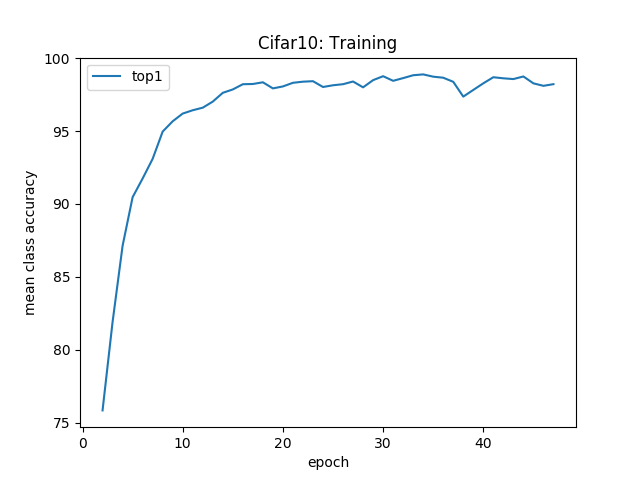
\includegraphics[width=1\textwidth]{\path/training.png} 
  \caption{Accuracy sul training set}
 \label{fig:training}
\end{subfigure}%
\begin{subfigure}{.5\textwidth}
  \centering
 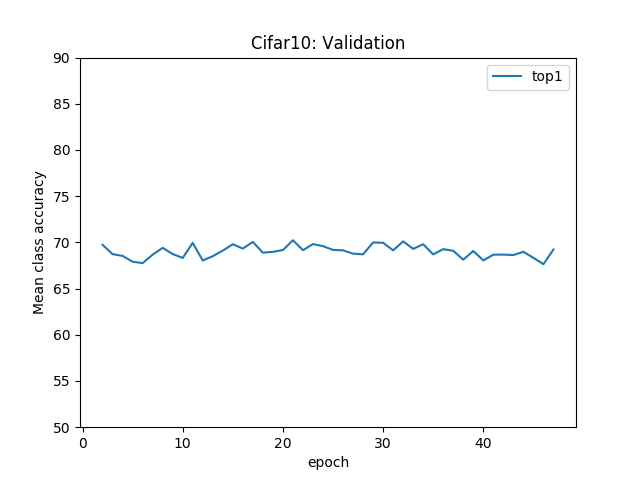
\includegraphics[width=1\textwidth]{\path/validation.png} 
  \caption{Accuracy sul validation set}
 \label{fig:validation}
\end{subfigure}
\caption{Performance della rete in training e validation}
\label{fig:cifar-compare}
\end{figure} 

\bigskip

\begin{figure}
\centering
\begin{subfigure}{.5\textwidth}
  \centering
 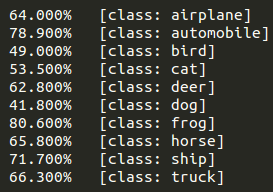
\includegraphics[width=1\textwidth]{\path/cifar-tanh.png} 
  \caption{Acc.= \textasciitilde 65\% f. di attivazione = TanH}
 \label{fig:training}
\end{subfigure}%
\begin{subfigure}{.5\textwidth}
  \centering
 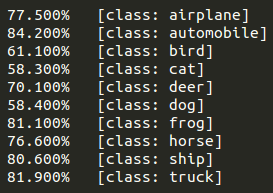
\includegraphics[width=1\textwidth]{\path/cifar-relu.png} 
  \caption{Acc.= \textasciitilde 73\% f. di attivazione = ReLU}
 \label{fig:validation}
\end{subfigure}
\caption{Percentuali di accuracy a seconda della funzione d'attivazione. La ReLU produce indubbiamente risultati migliori.}
\label{fig:relu}
\end{figure}
\\
%%%%% NEW PAGE FOR THE NEW FIGURES %%%% 
\newpage
\pagebreak
\medskip
\newpage

\begin{figure}[h!]
 \centering
 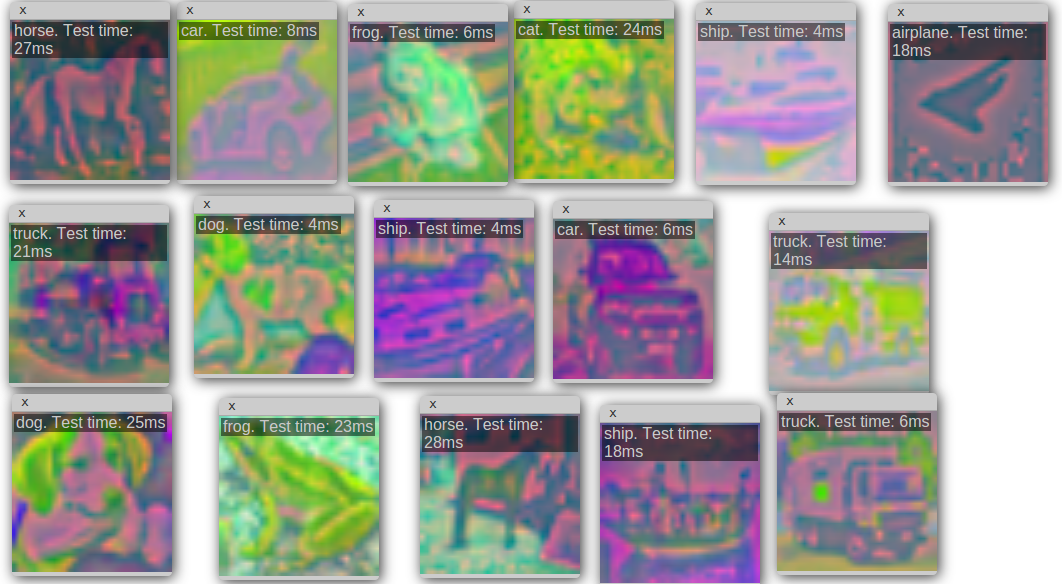
\includegraphics[width=1.0\textwidth]{\path/cifar-correct.png} 
 \caption{Esempi classificati correttamente}
 \label{fig:cifar-correct}
\end{figure}

\begin{figure}[h!]
 \centering
 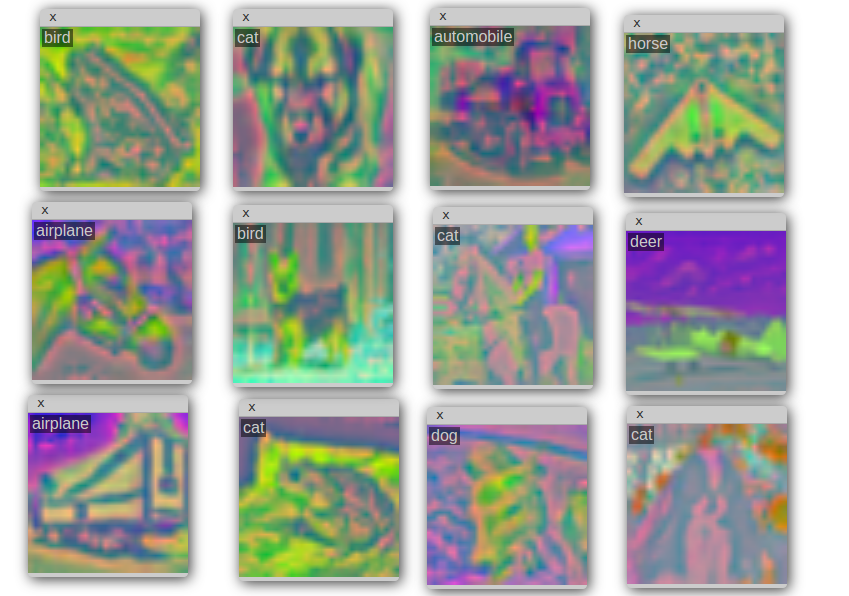
\includegraphics[width=1.0\textwidth]{\path/cifar-wrong.png} 
 \caption{Esempi classificati erroneamente}
 \label{fig:cifar-wrong}
\end{figure}
\\
Vedremo nel capitolo seguente un confronto dei risultati di una CNN con un'archittettura allo stato dell'arte testata sullo stesso dataset. 